% Section content template for individual Educative lessons
% This file contains the actual content for a specific section
% Generated from Educative API section content

% Section: High-Level Design of WhatsApp
% Section ID: 6728651831246848
% Section Slug: high-level-design-of-whatsapp
% Generated: 2025-12-08T15:00:18.819063

\subsection{High-level design}\label{nGpJdHb_QCmXWKp2Nctpd}
\\
At an abstract level, the high-level design consists of a chat server responsible for communication between the sender and the receiver. When a user wants to send a message to another user, both connect to the chat server. Both users send their messages to the chat server. The chat server then sends the message to the other intended user and also stores the message in the database.

\begin{figure}[htbp]
 \centering
 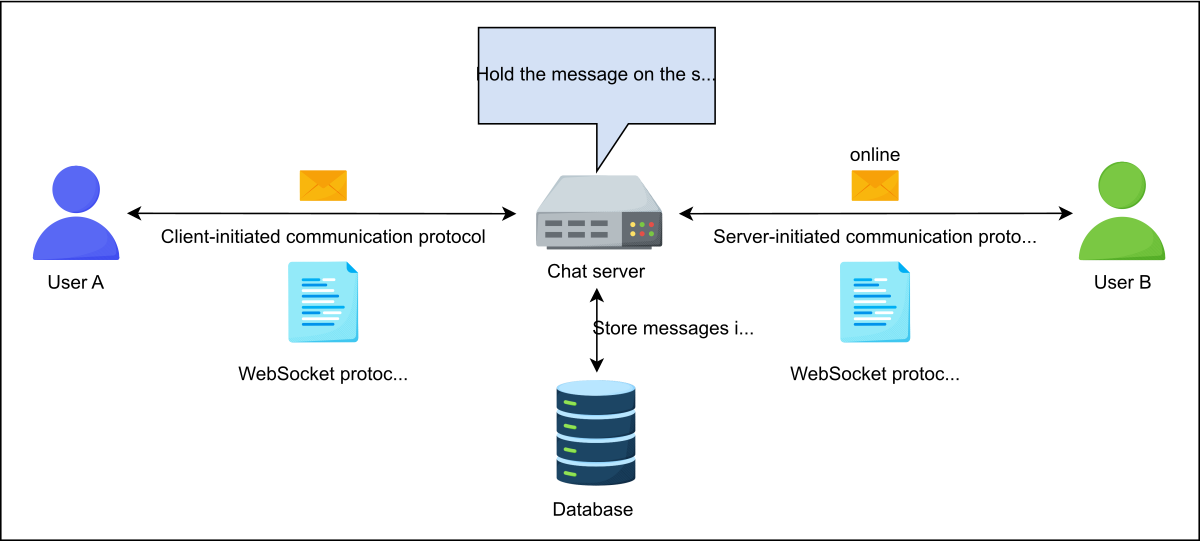
\includegraphics[width=0.5\textwidth]{Images/chapter_36/section_6728651831246848/6010869563916288.png}
 \caption{The high-level design of WhatsApp messenger}
\end{figure}

The following steps describe the communication between both clients:

\begin{enumerate}
\item
\protect\phantomsection\label{6TgiBuBvQ_Kadb95lRXbJ}
User A and user B create a communication channel with the chat server.
\item
\protect\phantomsection\label{NEpi_c0miIKB2MoZg9Zfr}
User A sends a message to the chat server.
\item
\protect\phantomsection\label{CTRVFOV2TZFFx8OOMJAGL}
Upon receiving the message, the chat server acknowledges back to user A.
\item
\protect\phantomsection\label{jWHsPlrjQZ-7jwYALvHa8}
The chat server sends the message to user B and stores the message in the database if the receiver\textquotesingle s status is offline.
\item
\protect\phantomsection\label{-fcQcv6Em0T2Fu-eYvndM}
User B sends an acknowledgment to the chat server.
\item
\protect\phantomsection\label{vXtfNWjEhVNBij6I_W7DF}
The chat server notifies user A that the message has been successfully delivered.
\item
\protect\phantomsection\label{WdynjMmYwLzeprfK-pGqZ}
When user B reads the message, the application notifies the chat server.
\item
\protect\phantomsection\label{ta-HIrpTc-tW0EGrQH-Ij}
The chat server notifies user A that user B has read the message.
\end{enumerate}
\\
The process is shown in the following illustrations:

\begin{figure}[htbp]
 \centering
 \begin{subfigure}[b]{0.48\textwidth}
 \centering
 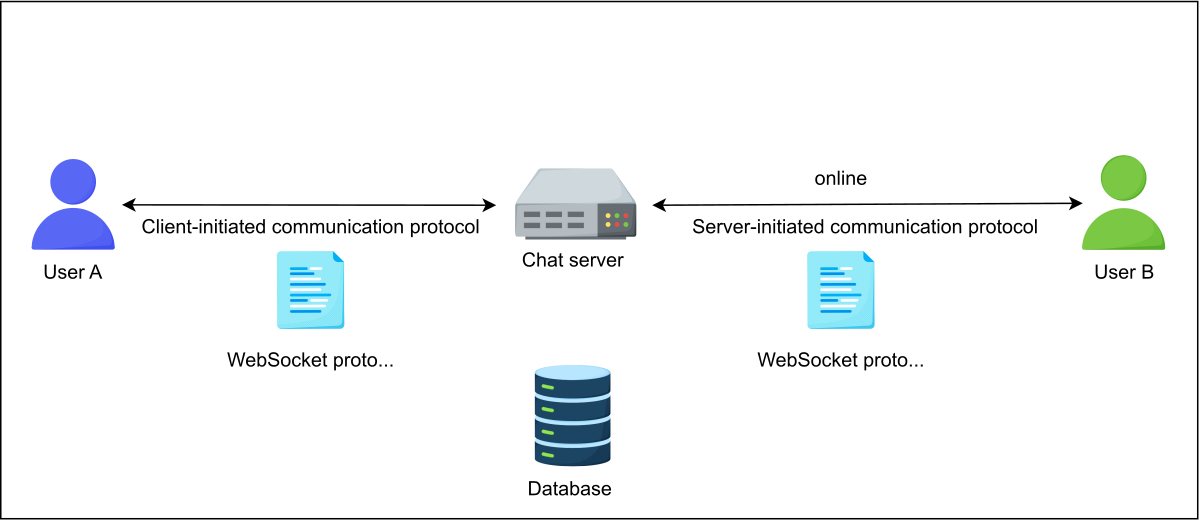
\includegraphics[width=\textwidth]{Images/chapter_36/section_6728651831246848/5981990119931904.png}
 \caption{User A and user B create connections with the chat server}
 \end{subfigure}
 \hfill
 \begin{subfigure}[b]{0.48\textwidth}
 \centering
 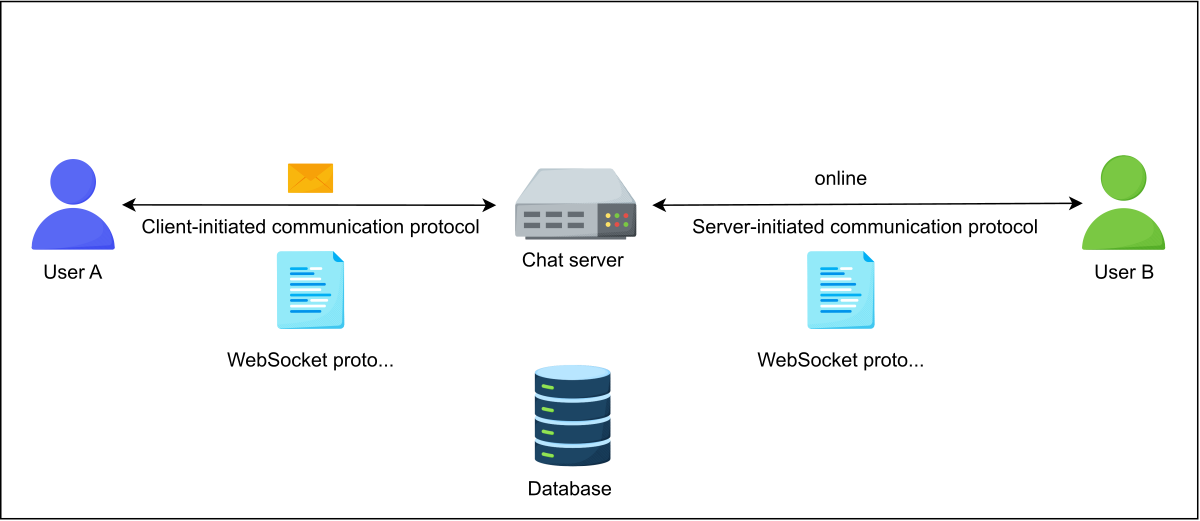
\includegraphics[width=\textwidth]{Images/chapter_36/section_6728651831246848/4619833541263360.png}
 \caption{User A sends a message to the chat server}
 \end{subfigure}
\end{figure}

\begin{figure}[htbp]
 \centering
 \begin{subfigure}[b]{0.48\textwidth}
 \centering
 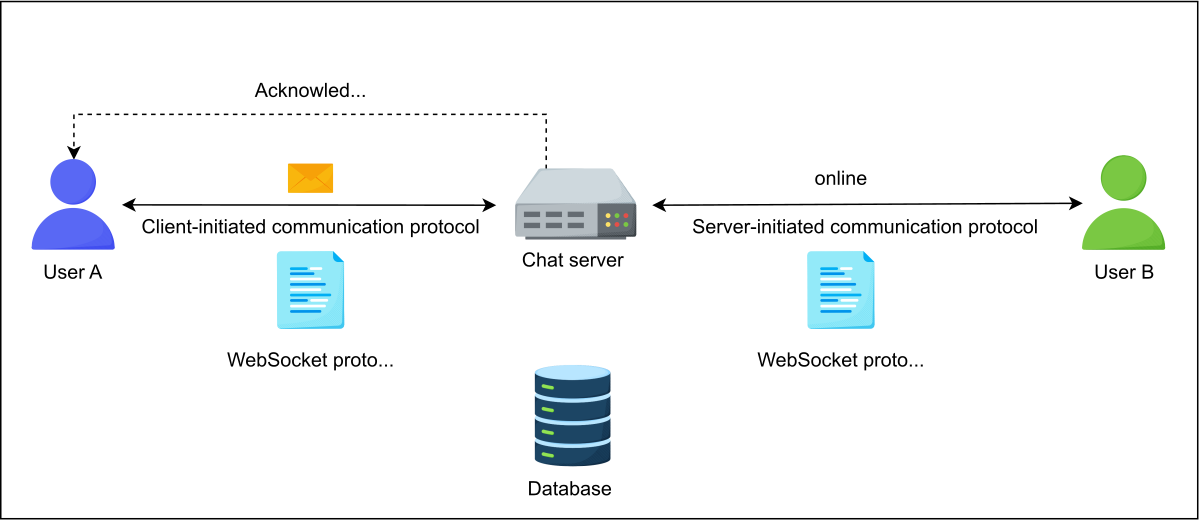
\includegraphics[width=\textwidth]{Images/chapter_36/section_6728651831246848/6314332894134272.png}
 \caption{Upon receiving the message, the chat server acknowledges back to user A}
 \end{subfigure}
 \hfill
 \begin{subfigure}[b]{0.48\textwidth}
 \centering
 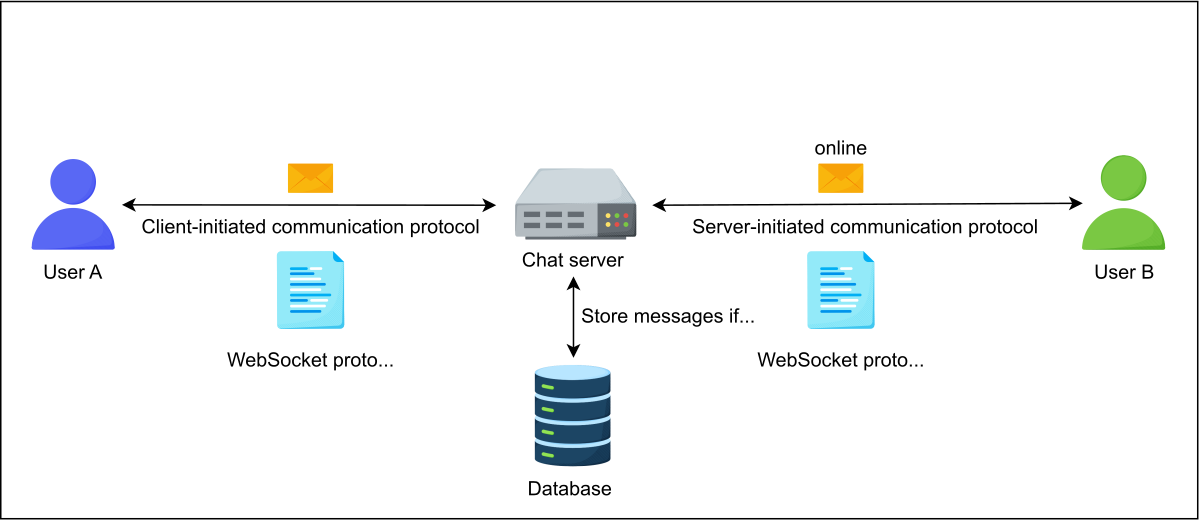
\includegraphics[width=\textwidth]{Images/chapter_36/section_6728651831246848/6561104182771712.png}
 \caption{The chat server sends the message to user B and stores the message in the database}
 \end{subfigure}
\end{figure}

\begin{figure}[htbp]
 \centering
 \begin{subfigure}[b]{0.48\textwidth}
 \centering
 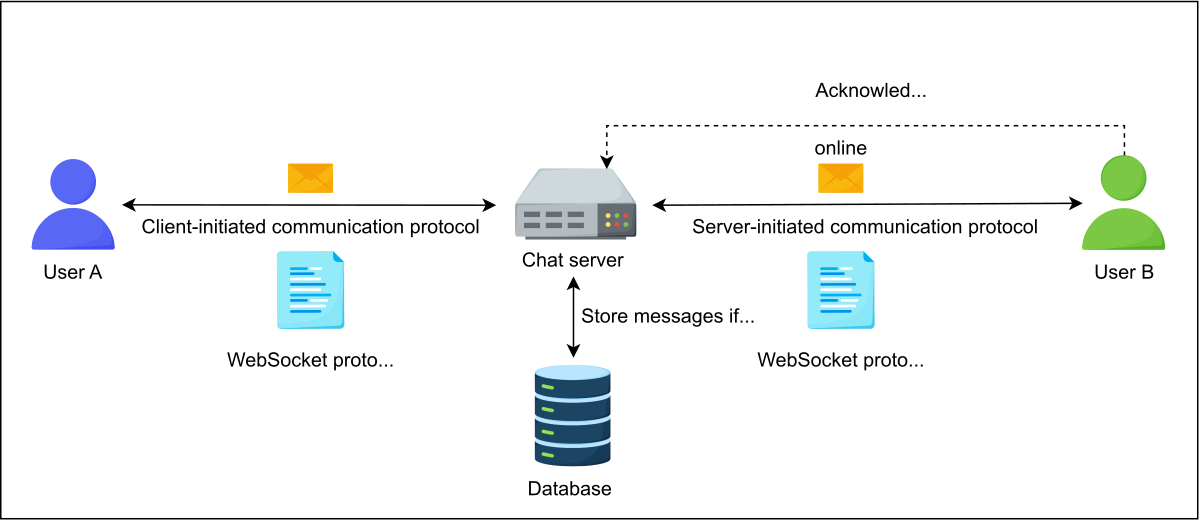
\includegraphics[width=\textwidth]{Images/chapter_36/section_6728651831246848/5600309496119296.png}
 \caption{User B sends an acknowledgment to the chat server}
 \end{subfigure}
 \hfill
 \begin{subfigure}[b]{0.48\textwidth}
 \centering
 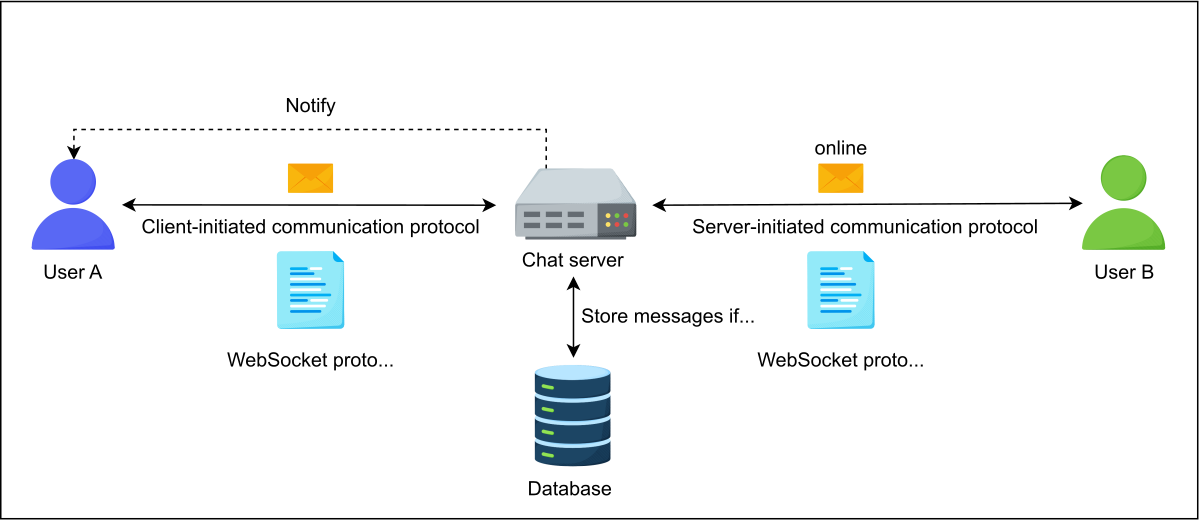
\includegraphics[width=\textwidth]{Images/chapter_36/section_6728651831246848/5435765171814400.png}
 \caption{The chat server notifies user A that the message has been successfully delivered}
 \end{subfigure}
\end{figure}

\begin{figure}[htbp]
 \centering
 \begin{subfigure}[b]{0.48\textwidth}
 \centering
 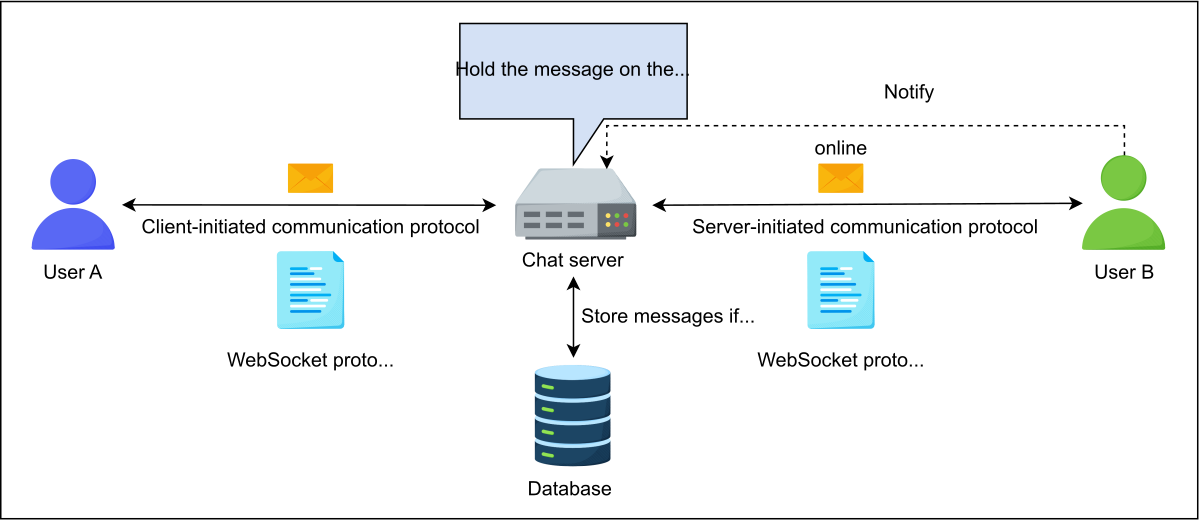
\includegraphics[width=\textwidth]{Images/chapter_36/section_6728651831246848/5640911298363392.png}
 \caption{When user B reads the message, the application notifies the chat server}
 \end{subfigure}
 \hfill
 \begin{subfigure}[b]{0.48\textwidth}
 \centering
 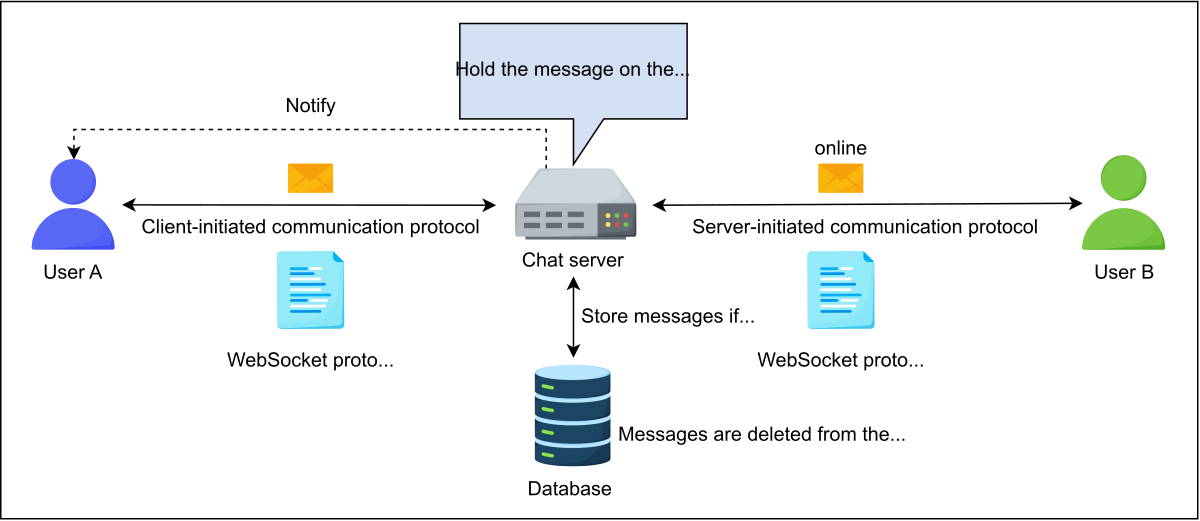
\includegraphics[width=\textwidth]{Images/chapter_36/section_6728651831246848/6412007748534272.png}
 \caption{The chat server notifies user A that user B has read the message}
 \end{subfigure}
\end{figure}

\subsection{API Design}\label{zEKzT2_kNlQPGvSNAAkTl}
\\
WhatsApp provides a vast amount of features to its users via different APIs. Some features are mentioned below:

\begin{itemize}
\item
\protect\phantomsection\label{D1mgDCAo_3eY0r7mLQHBX}
Send message
\item
\protect\phantomsection\label{wtKLRy6f8wo-gis3GEpJg}
Get message or receive message
\item
\protect\phantomsection\label{dKjvuRSBBb7wYBXpb6ojE}
Upload a media file or document
\item
\protect\phantomsection\label{Pltf2Wk489sqr9uToDxcY}
Download document or media file
\item
\protect\phantomsection\label{nDdsR8Uz-VF4xRwhYBvEU}
Send a location
\item
\protect\phantomsection\label{khkOf1aAWu4dhbgm3FE1W}
Send a contact
\item
\protect\phantomsection\label{pTrTn6FRgww6isT-VSd1_}
Create a status
\end{itemize}
\\
However, we'll discuss essential APIs related to the first four features.

\subsubsection{Send message}\label{N--nHT_Vytmqqoln9teaB}
\\
The \texttt{sendMessage} API is as follows:

\begin{lstlisting}[language=JavaScript]
sendMessage(message_ID, sender_ID, receiver_ID, type, text=none, media_object=none, document=none)
\end{lstlisting}

This API is used to send a \texttt{text} message from a sender to a receiver by making a POST API call to the \texttt{/messages} API endpoint. Generally , the sender's and receiver's IDs are their phone numbers. The parameters used in this API call are described in the following table:

\begin{table}[htbp]
\centering
\small
\adjustbox{max width=\textwidth}{
\begin{tabular}{|p{0.207\textwidth}|p{0.743\textwidth}|}
\hline
\textbf{Parameter} & \textbf{Description} \\
\hline
\hline
\texttt{message\_ID} & This is a unique identifier of the message sent. \\
\hline
\texttt{sender\_ID} & This is a unique identifier of the user who sends the message. \\
\hline
\texttt{reciever\_ID} & This is a unique identifier of the user who receives the message. \\
\hline
\texttt{type} & The default message \texttt{type} is text. This represents whether the sender sends a media file or a document. \\
\hline
\texttt{text} & This field contains the text that has to be sent as a message. \\
\hline
\texttt{media\_object} & This parameter is defined based on the type parameter. It represents the media file to be sent. \\
\hline
\texttt{document} & This represents the document file to be sent. \\
\hline
\end{tabular}
}
\end{table}

\subsubsection{Get message}\label{zUlkLeGu1gQM4TsyUDDGJ}
\\
The \texttt{getMessage} API is as follows:

\begin{lstlisting}[language=JavaScript]
getMessage(user_Id)
\end{lstlisting}

Using this API call, users can fetch all unread messages when they come online after being offline for some time.

\begin{table}[htbp]
\centering
\small
\adjustbox{max width=\textwidth}{
\begin{tabular}{|p{0.207\textwidth}|p{0.743\textwidth}|}
\hline
\textbf{Parameter} & \textbf{Description} \\
\hline
\hline
\texttt{user\_Id} & This is a unique identifier representing the user who has to fetch all unread messages. \\
\hline
\end{tabular}
}
\end{table}

\subsubsection{Upload media or document file}\label{n1nx_EyyZmpdcmfi_Vvg2}
\\
The \texttt{uploadFile} API is as follows:

\begin{lstlisting}[language=JavaScript]
uploadFile(file_type, file)
\end{lstlisting}

We can upload media files via the \texttt{uploadFile} API by making a POST request to the \texttt{/v1/media} API endpoint. A successful response returns an ID that's forwarded to the receiver. The maximum file size for media that can be uploaded is 16 MB, while the limit is 100 MB for a document.

\begin{table}[htbp]
\centering
\small
\adjustbox{max width=\textwidth}{
\begin{tabular}{|p{0.207\textwidth}|p{0.743\textwidth}|}
\hline
\textbf{Parameter} & \textbf{Description} \\
\hline
\hline
\texttt{file\_type} & This represents the type of file uploaded via the API call. \\
\hline
\texttt{file} & This contains the file being uploaded via the API call.~ \\
\hline
\end{tabular}
}
\end{table}

\subsubsection{Download a document or media file}\label{RJStTlMG3IjUuZXNgSr3r}
\\
The \texttt{downloadFile} API is as follows:

\begin{lstlisting}[language=JavaScript]
downloadFile(user_id, file_id)
\end{lstlisting}

The parameters of this API call are explained in the following table:

\begin{table}[htbp]
\centering
\small
\adjustbox{max width=\textwidth}{
\begin{tabular}{|p{0.207\textwidth}|p{0.743\textwidth}|}
\hline
\textbf{Parameter} & \textbf{Description} \\
\hline
\hline
\texttt{user\_id} & This is a unique identifier of the user who will download a file. \\
\hline
\texttt{file\_id} & This is a unique identifier of a file. It's generated while uploading a file via \texttt{uploadFile()} API call. The \texttt{downloadFile()} API call downloads the media file through this identifier. The client can find the \texttt{file\_id} by providing the file name to the server. That API call is not shown here. \\
\hline
\end{tabular}
}
\end{table}

In \href{https://www.educative.io/courses/grokking-the-system-design-interview/system-design-whatsapp}{introduction}, we stated that WhatsApp handled over 100 billion messages daily in 2020---a 54\% increase from 2018. If message volume continues to grow, how should the system scale to support billions of users efficiently? Use the interactive widget below to explain your approach.

In the next lesson, we'll focus on the detailed design of the WhatsApp system.

% End of section content